\chapter{Probabilistic methods}
\lbl{ch:prob}
\index{Aubrun, Guillaume}
\index{Nechita, Ion}

Much of this book is about characterization theorems for entropies,
diversities and means, and the conditions that characterize these
quantities are mostly functional%
%
\index{functional equation}
% 
equations.  In this chapter, we will see how to solve certain
functional equations using results from probability theory, following the
pioneering~2011 work of Aubrun and Nechita~\cite{AuNe}.  The technique is
demonstrated first with their startlingly simple characterization of the
$\ell^p$ norms, and then with a similar theorem for the power means,
different from the characterizations in Chapter~\ref{ch:mns}.

Functional equations are completely deterministic entities, with no
stochastic element.  How, then, can the power of probability theory be
brought to bear?

A simple analogy demonstrates the general idea.  Suppose that we want to
multiply out the expression
\[
(x + y)^{1000} = (x + y)(x + y) \cdots (x + y)
\]
as a sum of terms $x^a y^b$.  Which terms $x^a y^b$%
%
\index{binomial expansion} 
% 
appear, and how many of them are there?

The standard answer is, of course, that all the terms in the expansion
satisfy $a + b = 1000$ with $a, b \geq 0$, and that the number of such
terms is exactly $1000!/a!b!$.  But there is a different kind of answer:
that \emph{most} of the terms are of the form $x^a y^b$ where $a$ and $b$
are each \emph{about} $500$.  To see this, we can contemplate
the process of multiplying out the brackets, in which one has to go through
all $2^{1000}$ ways of making $1000$ choices between $x$ and $y$.  If we
flip a fair coin%
%
\index{coin!toss}
% 
$1000$ times, we usually obtain about $500$ each of
heads and tails, and this is the reason why most values of $a$ and $b$ are
about $500$.

This alternative answer has several distinguishing features.  It is
approximate, and the approximation is obtained by probabilistic reasoning.
Depending on the degree of precision required for the purpose at hand, and
depending on the meanings of `most' and `about', this approximation may be
all that we need.  It is also simpler than the first, precise, answer.  All
of these features are also displayed by the probabilistic method described
in this chapter.

For us, the key theorem from probability theory is a variational formula
for the moment generating function (Section~\ref{sec:mgfs}).  Conceptually,
this formula can be understood as the convex conjugate of Cram\'er's large
deviation theorem (Section~\ref{sec:large}).  The probabilistic method is
applied to characterize the $\ell^p$ norms in Section~\ref{sec:mult-norms}
and the power means in Section~\ref{sec:mult-means}.

This chapter assumes some basic probability theory, but not much more than
the language of random variables.  The most technically sophisticated part,
Section~\ref{sec:large}, is for context only and is not logically necessary
for anything that follows.


\section{Moment generating functions}
\lbl{sec:mgfs}


In this short section, we give a variational formula for the moment
generating function of any real random variable.  It can be found in Cerf%
% 
\index{Cerf, Rapha\"el}
% 
and Petit~\cite{CePe},% 
% 
\index{Petit, Pierre}
% 
who call it a `dual equality', a name explained in
the next section.  The proof given here is different from theirs.

Let $X$ be a real random variable.  The \demph{moment%
%
\index{moment generating function}
%
generating function}
of $X$ is the function 
\[
\begin{array}{cccc}
m_X\from        &\R             &\to            &[0, \infty]            \\
                &\lambda        &\mapsto        &\Ex\bigl(e^{\lambda X}\bigr),
\ntn{mgf}
\end{array}
\]
where $\Ex$ denotes expected value.

\begin{thm}
\lbl{thm:cp}
Let $X, X_1, X_2, \ldots$ be independent identically distributed real
random variables.  Write
\[
\ovln{X}_r
=
\tfrac{1}{r}(X_1 + \cdots + X_r)
\ntn{runningmean}
\]
($r \geq 1$).  Then
% 
\begin{equation}
\lbl{eq:cp}
m_X(\lambda)
=
\sup_{x \in \R, \ r \geq 1}
e^{\lambda x} \, \Pr\bigl(\ovln{X}_r \geq x\bigr)^{1/r} 
\end{equation}
% 
for all $\lambda \geq 0$, where the supremum is over all real $x$ and
positive integers $r$.
\end{thm}

We allow infinite values on either side of equation~\eqref{eq:cp}.

The proof, given below, uses the elementary result of probability theory
known as \demph{Markov's inequality} (Grimmett and Stirzaker~\cite{GrSt},
Lemma~7.2(7)):

\begin{lemma}[Markov] 
\lbl{lemma:markov}%
\index{Markov's inequality}%
%
Let $Z$ be a random variable taking nonnegative real values.  Then for all
$z \in \R$,
\[
\Ex(Z) \geq z \cdot \Pr(Z \geq z).
\]
\end{lemma}

This is intuitively clear: if one third of the people in a room are at
least 60 years old, then the mean age\index{age} is at least 20.

For the proof, we use some standard notation: given $S \sub \R$, let
$I_S \from \R \to \R$ denote the \demph{indicator%
%
\index{indicator function}
% 
function} (or \demph{characteristic%
%
\index{characteristic function}
% 
function}) of $S$, defined by
\[
I_S(x)
=
\begin{cases}
1       &\text{if } x \in S,    \\
0       &\text{otherwise}.
\end{cases}
\ntn{indicator}
\]

\begin{proof}
We have
\[
Z 
\geq 
z \cdot I_{[z, \infty)}(Z),
\]
by considering the cases $Z \geq z$ and $Z < z$ separately.  Hence
\[
\Ex(Z) 
\geq
\Ex\bigl( 
z \cdot I_{[z, \infty)}(Z)
\bigr)
=
z \cdot \Pr(Z \geq z).
\]
% as required.
\end{proof}

\begin{pfof}{Theorem~\ref{thm:cp}}
Let $\lambda \geq 0$.  We prove equation~\eqref{eq:cp} by showing that each
side is greater than or equal to the other.

First we show that 
\[
m_X(\lambda) 
\geq
\sup_{x \in \R, \ r \geq 1}
e^{\lambda x} \, \Pr\bigl(\ovln{X}_r \geq x\bigr)^{1/r}.
\]
Let $x \in \R$ and $r \geq 1$; we must show that
\[
\Ex\bigl(e^{\lambda X}\bigl)^r
\geq
e^{r\lambda x} \, \Pr\bigl(\ovln{X}_r \geq x\bigr).
\]
And indeed, 
% 
\begin{align}
\Ex\bigl(e^{\lambda X}\bigr)^r    &
=
\Ex\bigl(e^{\lambda(X_1 + \cdots + X_r)}\bigr)
\lbl{eq:cp-1} \\
&
=
\Ex\bigl(e^{r\lambda\ovln{X}_r}\bigr)
\nonumber       \\
&
\geq
e^{r\lambda x} \,
\Pr\bigl(
e^{r\lambda\ovln{X}_r} \geq e^{r\lambda x}
\bigr)
\lbl{eq:cp-3} \\
&
\geq
e^{r\lambda x} \, \Pr\bigl(\ovln{X}_r \geq x\bigr),
\lbl{eq:cp-4}
\end{align}
% 
where~\eqref{eq:cp-1} holds because $X, X_1, X_2, \ldots$ are independent
and identically distributed, \eqref{eq:cp-3}~follows from Markov's
inequality, and \eqref{eq:cp-4}~holds because $e^{r\lambda y}$ is
increasing in $y \in \R$.

Now we prove the opposite inequality, 
% 
\begin{equation}
\lbl{eq:cp-hard}
m_X(\lambda) 
\leq
\sup_{x \in \R, \ r \geq 1}
e^{\lambda x} \, \Pr\bigl(\ovln{X}_r \geq x\bigr)^{1/r}.
\end{equation}
% 
The strategy is to show that $\Ex\bigl( e^{\lambda X} I_{[-a, a]}(X)
\bigr)$ is bounded above by the right-hand side of~\eqref{eq:cp-hard} for
each $a > 0$, then to deduce that the same is true of $\Ex(e^{\lambda X}) =
m_X(\lambda)$ itself.

Let $a > 0$ and $\delta > 0$ be real numbers.  We can choose an integer $d
\geq 1$ and real numbers $v_0, \ldots, v_d$ such that
\[
-a = v_0 < v_1 < \cdots < v_d = a
\]
and $v_k \leq v_{k - 1} + \delta$ for all $k \in \{1, \ldots, d\}$.  Then
for all integers $s \geq 1$, 
% 
\begin{align}
\Ex\bigl(
e^{\lambda X} I_{[-a, a]}(X) \bigr)^s   &
=
\Ex\Bigl(
e^{\lambda X_1} I_{[-a, a]}(X_1) 
\cdots
e^{\lambda X_s} I_{[-a, a]}(X_s)
\Bigr)
\lbl{eq:cph-1}        \\
&
\leq
\Ex\Bigl(
e^{s\lambda\ovln{X}_s} I_{[-a, a]}\bigl(\ovln{X}_s\bigr)
\Bigr)
\lbl{eq:cph-2}        \\
&
\leq
\sum_{k = 1}^d 
\Pr\bigl(v_{k - 1} \leq \ovln{X}_s \leq v_k\bigr) e^{s\lambda v_k}
\lbl{eq:cph-3}        \\
&
\leq
\sum_{k = 1}^d \Pr\bigl(\ovln{X}_s \geq v_{k - 1}\bigr) 
e^{s\lambda v_{k - 1}} e^{s \lambda \delta}     
\lbl{eq:cph-4}        \\
&
\leq
e^{s\lambda\delta} d \, \sup_{x \in \R} \, 
e^{s\lambda x}\, \Pr\bigl(\ovln{X}_s \geq x\bigr),
\nonumber
\end{align}
% 
where~\eqref{eq:cph-1} holds because $X, X_1, X_2, \ldots$ are independent
and identically distributed, \eqref{eq:cph-2}~holds because the mean of a
collection of numbers in the interval $[-a, a]$ also belongs to that
interval, \eqref{eq:cph-3}~follows from the definition of expected value,
and~\eqref{eq:cph-4} follows from the defining properties of $v_0, \ldots,
v_d$.  Hence
% 
\begin{align*}
\Ex\bigl(
e^{\lambda X} I_{[-a, a]}(X) 
\bigr)  &
\leq
e^{\lambda\delta} d^{1/s} \,
\,\sup_{x \in \R}\,
e^{\lambda x} \, \Pr\bigl(\ovln{X}_s \geq x\bigr)^{1/s}      \\
&
\leq
e^{\lambda \delta} d^{1/s}\,
\,\sup_{x \in \R, \ r \geq 1} \,
e^{\lambda x} \, \Pr\bigl(\ovln{X}_r \geq x\bigr)^{1/r}.
\end{align*}
% 
This holds for all real $\delta > 0$ and integers $s \geq 1$, so we can let
$\delta \to 0$ and $s \to \infty$, which gives
% 
% \begin{equation}
% \lbl{eq:cp-intvl}
\[
\Ex\bigl(
e^{\lambda X} I_{[-a, a]}(X) 
\bigr)  
\leq
\sup_{x \in \R, \ r \geq 1} 
e^{\lambda x} \, \Pr\bigl(\ovln{X}_r \geq x\bigr)^{1/r}.
\]
% \end{equation}
% 
Finally, letting $a \to \infty$ and using the monotone convergence theorem
gives the desired inequality~\eqref{eq:cp-hard}.
% 
% by the monotone convergence theorem,
% \[
% \Ex\bigl(
% e^{\lambda X} I_{[-a, a]}(X) 
% \bigr)  
% \to
% \Ex(e^{\lambda X}) = m_X(\lambda)
% \]
% as $a \to \infty$.
% 
\end{pfof}

The following example is the only instance of Theorem~\ref{thm:cp} that we
will need. 


\begin{example}
\lbl{eg:cp-fin}
Let $n \geq 1$ and $c_1, \ldots, c_n \in \R$.  Let $X, X_1, X_2, \ldots$ be
independent random variables with distribution $\tfrac{1}{n} \sum_{i = 1}^n
\delta_{c_i}$, where $\delta_c$ denotes the point mass at a real number
$c$. Thus, the random variables take values $c_1, \ldots, c_n$ with
probability $1/n$ each, adding probabilities if there are repeats among the
$c_i$.  For instance, if $n = 3$ and $(c_1, c_2, c_3) = (7, 7, 8)$, then
$X$ takes value $7$ with probability $2/3$ and $8$ with probability $1/3$.

The moment generating function of $X$ is given by
\[
m_X(\lambda)
=
\tfrac{1}{n}(e^{c_1 \lambda} + \cdots + e^{c_n \lambda})
\]
($\lambda \in \R$).  On the other hand, for $r \geq 1$,
\[
\Pr\bigl(\ovln{X}_r \geq x\bigr) 
=
\tfrac{1}{n^r} 
\bigl|\bigl\{
(i_1, \ldots, i_r) \such c_{i_1} + \cdots + c_{i_r} \geq rx
\bigr\}\bigr|.
\]
Hence by Theorem~\ref{thm:cp}, for all $\lambda \geq 0$, 
% 
\begin{equation}
\lbl{eq:cp-fin}
e^{c_1\lambda} + \cdots + e^{c_n\lambda}
=
\sup_{x \in \R, \ r \geq 1}
e^{\lambda x} 
\bigl|\bigl\{
(i_1, \ldots, i_r) \such c_{i_1} + \cdots + c_{i_r} \geq rx
\bigr\}\bigr|^{1/r}.
\end{equation}
% 
This is a completely deterministic statement about real numbers $c_1,
\ldots, c_n, \lambda$.
\end{example}

Theorem~\ref{thm:cp} gives the value of $m_X(\lambda)$ for $\lambda \geq 0$
only, but it is easy to deduce the value for negative $\lambda$:

\begin{cor}
\lbl{cor:cp-neg}
In the context of Theorem~\ref{thm:cp},
\[
m_X(\lambda)
=
\sup_{x \in \R, \ r \geq 1} 
e^{\lambda x} \, \Pr\bigl(\ovln{X}_r \leq x\bigr)^{1/r}
\]
for all $\lambda \leq 0$.
\end{cor}

\begin{proof}
Apply Theorem~\ref{thm:cp} to $-X$ and $-\lambda$, renaming $x$ as $-x$.
\end{proof}


\section{Large deviations and convex duality}
\lbl{sec:large}
\index{large deviations}

This section is not logically necessary for anything that follows, but
places the moment generating function formula of Theorem~\ref{thm:cp} into
a wider context.  Briefly put, that formula is the convex conjugate of
Cram\'er's large deviation theorem.  Here we explain what this means and
why it is true. 


\subsection*{Cram\'er's theorem}
\index{Cramer, Harald@Cram\'er, Harald}

Let $X, X_1, X_2, \ldots$ be independent identically distributed real
random variables, with mean $\mu$, say.  Given $x \in \R$, what can be said
about $\Pr\bigl(\ovln{X}_r \geq x\bigr)$ for large integers $r$?

The law%
%
\index{law of large numbers} 
% 
of large numbers implies that
\[
\Pr\bigl(\ovln{X}_r \geq x\bigr)
\to
\begin{cases}
1       &\text{if } x < \mu,    \\
0       &\text{if } x > \mu
\end{cases}
\]
as $r \to \infty$ (assuming that $\Ex(\mg{X})$ is finite).  However, it is
silent on the question of how \emph{fast} $\Pr\bigl(\ovln{X}_r \geq
x\bigr)$ converges as $r \to \infty$.

Consider, then, the central%
%
\index{central limit theorem} 
% 
limit theorem.  Loosely, this states that when $r$ is large, the
distribution of $\ovln{X}_r$ is approximately normal.%
%
\index{normal distribution}  
% 
This enables us to
estimate $\Pr\bigl(\ovln{X}_r \geq x\bigr)$ for large $r$; but again, it
does not help us with the \emph{rate} of convergence.

More exactly, assume without loss of generality that $\mu = 0$.  Then for
each $r \geq 1$, the random variable
\[
\sqrt{r}\,\ovln{X}_r
=
\frac{1}{\sqrt{r}}(X_1 + \cdots + X_r)
\]
has mean $0$ and the same variance ($\sigma^2$, say) as $X$.  The central
limit theorem states that as $r \to \infty$, the distribution of
$\sqrt{r}\,\ovln{X}_r$ converges to the normal distribution with mean $0$
and variance $\sigma^2$.  This gives a way of estimating the probability
\[
\Pr\Bigl(
\tfrac{1}{\sqrt{r}} (X_1 + \cdots + X_r) \geq x
\Bigr)
=
\Pr\Bigl( \ovln{X}_r \geq \tfrac{x}{\sqrt{r}} \Bigr)
\]
for any $x \in \R$ and large integer $r$.  But the original question was
about $\Pr\bigl(\ovln{X}_r \geq x\bigr)$, not $\Pr\bigl(\ovln{X}_r \geq
x/\sqrt{r}\bigr)$.  In other words, we are interested in larger deviations
from the mean than those addressed by the central limit theorem.

So, neither the law of the large numbers nor the central limit theorem
tells us the rate of convergence of $\Pr\bigl(\ovln{X}_r \geq x\bigr)$ as
$r \to \infty$.  But large deviation theory does.  Roughly speaking, the
basic fact is that for each $x \in \R$ there is a constant $k(x) \in [0,
  1]$ such that
\[
\Pr\bigl(\ovln{X}_r \geq x\bigr) 
\approx
k(x)^r
\]
when $r$ is large.  If $x > \mu$ then $k(x) < 1$, so the decay of
$\Pr\bigl(\ovln{X}_r \geq x\bigr)$ as $r \to \infty$ is exponential.  The
precise result is this.

\begin{thm}[Cram\'er]
\lbl{thm:cramer}%
\index{Cramer, Harald@Cram\'er, Harald}%
% 
Let $X, X_1, X_2, \ldots$ be independent identically distributed real
random variables, and let $x \in \R$.  Then the limit
\[
\lim_{r \to \infty} \Pr\bigl(\ovln{X}_r \geq x\bigr)^{1/r}
\]
exists and is equal to
\[
\inf_{\lambda \geq 0} \frac{\Ex(e^{\lambda X})}{e^{\lambda x}}.
\]
\end{thm}

Part of this statement is an easy consequence of Markov's%
%
\index{Markov's inequality} 
% 
inequality.  Indeed, we used Markov's inequality in
equations~\eqref{eq:cp-1}--\eqref{eq:cp-4} to show that
\[
\Pr\bigl(\ovln{X}_r \geq x\bigr)^{1/r} 
\leq 
\frac{\Ex(e^{\lambda X})}{e^{\lambda x}}
\]
for each $r \geq 1$ and $\lambda \geq 0$, so if the limit in Cram\'er's
theorem does exist then it is at most the stated infimum.  We do not prove
Cram\'er's theorem here, but a short proof can be found in Cerf%
%
\index{Cerf, Rapha\"el}
%
and Petit~\cite{CePe}%
%
\index{Petit, Pierre} 
% 
(who deduce it from Theorem~\ref{thm:cp} using the convex duality that we
are about to discuss), or see standard probability texts such as Grimmett
and Stirzaker (\cite{GrSt}, Theorem~5.11(4)).

\begin{example}
When $X$ is distributed normally%
% 
\index{normal distribution}
% 
with mean $\mu$ and variance $\sigma^2$,
its moment generating function is
\[
\Ex\bigl(e^{\lambda X}\bigr)
=
\exp\bigl(\lambda\mu + \hlf \lambda^2 \sigma^2\bigr).
\]
Hence
\[
\frac{\Ex\bigl(e^{\lambda X}\bigr)}{e^{\lambda x}}
=
\exp\bigl(
\hlf \sigma^2 \cdot \lambda^2 - (x - \mu) \cdot \lambda
\bigr).
\]
Minimizing $\Ex(e^{\lambda X})/e^{\lambda x}$ over $\lambda \geq 0$
therefore reduces to the routine task of minimizing a quadratic.  This
done, Cram\'er's theorem gives
\[
\lim_{r \to \infty} \Pr\bigl(\ovln{X}_r \geq x\bigr)^{1/r}
=
\begin{cases}
\displaystyle
1       &\text{if } x \leq \mu, \\
\displaystyle
\exp \Biggl( - \frac{(x - \mu)^2}{2\sigma^2} \Biggr)      &
\text{if } x \geq \mu.
\end{cases}
\]
As one would expect, this is a decreasing function of $x$ but an increasing
function of both $\mu$ and $\sigma$.
\end{example}

As this example suggests, it is natural to split Cram\'er's theorem into
two cases, according to whether $x$ is greater than or less than $\Ex(X)$:

\begin{cor}
\lbl{cor:cramer-cases}
Let $X, X_1, X_2, \ldots$ be independent identically distributed real
random variables.  
% 
\begin{enumerate}
\item 
\lbl{part:cramer-cases-R}
For all $x \geq \Ex(X)$,
\[
\lim_{r \to \infty} \Pr\bigl(\ovln{X}_r \geq x\bigr)^{1/r}
=
\inf_{\lambda \in \R} 
\frac{\Ex\bigl(e^{\lambda X}\bigr)}{e^{\lambda x}},
\]
and for all $x \leq \Ex(X)$,
\[
\lim_{r \to \infty} \Pr\bigl(\ovln{X}_r \leq x\bigr)^{1/r}
=
\inf_{\lambda \in \R} 
\frac{\Ex\bigl(e^{\lambda X}\bigr)}{e^{\lambda x}}.
\]
(Note that both infima are over \emph{all} $\lambda \in \R$, in contrast to 
Theorem~\ref{thm:cramer}.)

\item
\lbl{part:cramer-cases-1}
For all $x \leq \Ex(X)$,
\[
\lim_{r \to \infty} \Pr\bigl(\ovln{X}_r \geq x\bigr)^{1/r} 
=
1,
\]
and for all $x \geq \Ex(X)$,
\[
\lim_{r \to \infty} \Pr\bigl(\ovln{X}_r \leq x\bigr)^{1/r} 
=
1.
\]
\end{enumerate}
\end{cor}

\begin{proof}
For both parts, we use the inequality $e^x \geq 1 + x$, which implies that
% 
\begin{equation}
\lbl{eq:cc-1}
\frac{\Ex\bigl(e^{\lambda X}\bigr)}{e^{\lambda x}}
=
\Ex\bigl(e^{\lambda(X - x)}\bigr)
\geq
\Ex\bigl(1 + \lambda(X - x)\bigr)
=
1 + \lambda\bigl(\Ex(X) - x\bigr)  
\end{equation}
% 
for all $\lambda, x \in \R$.  We also use the fact that
% 
\begin{equation}
\lbl{eq:cc-2}
\frac{\Ex\bigl(e^{0X}\bigr)}{e^{0x}} = 1
\end{equation}
% 
for all $x \in \R$.

For~\bref{part:cramer-cases-R}, let $x \geq \Ex(X)$.  When $\lambda \leq
0$, \eqref{eq:cc-1} and~\eqref{eq:cc-2} give
% 
\begin{equation}
\lbl{eq:cc-3}
\frac{\Ex\bigl(e^{\lambda X}\bigr)}{e^{\lambda x}}
\geq
1 
=
\frac{\Ex\bigl(e^{0 X}\bigr)}{e^{0 x}},
\end{equation}
% 
so the infimum in Theorem~\ref{thm:cramer} is unchanged if we allow
$\lambda$ to range over all of $\R$.  This gives the first equation
of~\bref{part:cramer-cases-R}.  The second follows by applying the first to
$-X$ and $-x$, renaming $\lambda$ as $-\lambda$.

For~\bref{part:cramer-cases-1}, let $x \leq \Ex(X)$.  When $\lambda \geq
0$, \eqref{eq:cc-1} and~\eqref{eq:cc-2} again imply~\eqref{eq:cc-3}, so the
infimum in Theorem~\ref{thm:cramer} is $1$.  This gives the first equation
of~\bref{part:cramer-cases-1}, and again, the second follows by applying the
first to $-X$ and $-x$.
\end{proof}


\subsection*{Convex duality}
\index{convex!duality}

To relate the formula for moment generating functions in
Theorem~\ref{thm:cp} to Cram\'er's theorem, we use the principle of convex
duality.

\begin{defn}
Let $f \from \R \to [-\infty, \infty]$ be a function.  Its
\demph{convex%
%
\index{convex!conjugate}
%  
conjugate} or \demph{Legendre--Fenchel%
%
\index{Legendre--Fenchel transform}
% 
transform} is the function $f^*
\from \R \to [-\infty, \infty]$ defined by
% 
\begin{equation}
\lbl{eq:defn-conj}
f^*(\lambda) = \sup_{x \in \R} \bigl( \lambda x - f(x) \bigr).
\end{equation}
\end{defn}

The theory of convex conjugates is developed thoroughly in texts such as
Borwein and Lewis~\cite{BoLe} and Rockafellar~\cite{Rock}.  Here we give a
brief summary tailored to our needs.

\begin{examples}
\lbl{egs:conj}
\begin{enumerate}
\item 
\lbl{eg:conj-diff}
Let $f \from \R \to \R$ be a differentiable function such that $f' \from \R
\to \R$ is an increasing bijection. 
% (or equivalently, $f'$ is continuous,
% strictly increasing, and unbounded both above and below).  
Then for each
$\lambda \in \R$, the function 
\[
x \mapsto \lambda x - f(x)
\]
has a unique critical point $x_\lambda = {f'}^{-1}(\lambda)$, which is also
the unique global maximum.  Hence
\[
f^*(\lambda) = \lambda x_\lambda - f(x_\lambda).
\]
In graphical terms, for each real number $\lambda$, there is a unique
tangent line to the graph of $f$ with gradient (slope) $\lambda$, and its
equation is
\[
y = \lambda x - f^*(\lambda)
\]
(Figure~\ref{fig:conj-diff}).  Thus, $f^*(\lambda)$ is the negative of the
$y$-intercept of this tangent line.  The convex conjugate $f^*$ therefore
describes $f$ in terms of its envelope of tangent lines.

\begin{figure}
\centering
\lengths
\begin{picture}(120,50)
\cell{60}{25}{c}{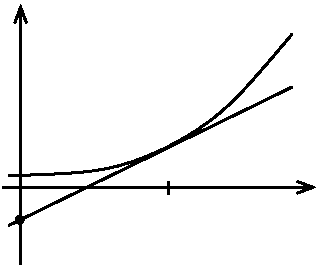
\includegraphics[height=50\unitlength]{conjugate}}
\cell{88}{11.7}{c}{$x$}
% \cell{30}{40}{c}{$f(x)$}
\cell{76}{40}{c}{$f(x)$}
\cell{82}{30}{l}{gradient $\lambda$}
\cell{44}{7}{c}{$(0, -f^*(\lambda))$}
\cell{62}{11.5}{c}{$x_\lambda$}
\end{picture}
\caption{The relationship between a differentiable function $f$ and its
  convex conjugate $f^*$ (Example~\ref{egs:conj}\bref{eg:conj-diff}).}
\lbl{fig:conj-diff}
\end{figure}

\item
Let $p, q \in (1, \infty)$ be conjugate exponents, that is, $1/p + 1/q =
1$.  Then the functions $x \mapsto \mg{x}^p/p$ and $x \mapsto
\mg{x}^q/q$ are convex conjugate to one another, as can be shown
using~\bref{eg:conj-diff}.

\item
More generally, let $f, g \from \R \to \R$ be differentiable functions such
that $f'$ and $g'$ are increasing and $f'(0) = 0 = g'(0)$.  It can be shown
that if $f', g' \from \R \to \R$ are mutually inverse then $f$ and $g$ are
mutually convex conjugate (Section~I.9 of Zygmund~\cite{Zygm}).  At this
level of generality, convex duality has also been called Young
complementarity or Young%
% 
\index{Young duality} 
% 
duality, as in~\cite{Zygm} or Section~14D of Arnold~\cite{Arno}.
\end{enumerate}
\end{examples}

% These examples and the results that follow reveal the reason for
% the word `convex' in `convex conjugate'.

\begin{lemma}
\lbl{lemma:conj-cvx}
For every function $f \from \R \to [-\infty, \infty]$, the convex conjugate
$f^* \from \R \to [-\infty, \infty]$ is convex.\index{convex!function}
\end{lemma}

Before we can prove this, we need to state what it means for a function
into $[-\infty, \infty]$ to be convex.  If the function takes only finite
values, or takes $\infty$ but not $-\infty$ as a value, or vice versa, then
the meaning is clear.  If it takes both $-\infty$ and $\infty$ as values
then the matter is more delicate; a careful treatment can be found in
Section~2.2.2 of Willerton~\cite{WillLFT} (ultimately derived from
Lawvere~\cite{LawvSCC}).  Fortunately, we can avoid the issue here.  If $f
\equiv \infty$ then $f^* \equiv -\infty$, in which case $f^*$ is convex by
any reasonable definition.  Otherwise, $f^*$ never takes the value
$-\infty$, so the problem does not arise.

\begin{proof}
Let $\lambda, \mu \in \R$ and $p \in [0, 1]$.  Then
% 
\begin{align*}
f^*\bigl(p\lambda + (1 - p)\mu\bigr)    &
=
\sup_{x \in \R} \bigl(
p\lambda x + (1 - p)\mu x - f(x)
\bigr)  \\
&
=
\sup_{x \in \R} \bigl(
p [\lambda x - f(x)] + (1 - p)[\mu x - f(x)]
\bigr)  \\
&
\leq
\sup_{y, z \in \R} \bigl(
p [\lambda y - f(y)] + (1 - p)[\mu z - f(z)]
\bigr)  \\
&
=
p f^*(\lambda) + (1 - p)f^*(\mu),
\end{align*}
% 
as required.
\end{proof}

The examples above suggest that often $f^{**} = f$.  By
Lemma~\ref{lemma:conj-cvx}, this cannot be true unless $f$ is convex.  For
finite-valued $f$, that is the \emph{only} restriction:

\begin{thm}[Legendre--Fenchel]
\lbl{thm:lf}%
\index{Legendre--Fenchel transform}%
\index{Fenchel, Werner}%
% 
Let $f \from \R \to \R$ be a convex function.  Then $f^{**} = f$.
\end{thm}

\begin{proof}
This standard result can be found in textbooks on convex analysis; see
Theorem~4.2.1 of Borwein and Lewis~\cite{BoLe} or Section~14C of
Arnold~\cite{Arno}, for instance.  A proof is also included as
Appendix~\ref{sec:cvx-du}.
\end{proof}

\begin{remarks}
\begin{enumerate}
\item 
Theorem~\ref{thm:lf} is a very special case of the full Legendre--Fenchel
theorem.  For a start, we restricted to finite-valued functions, thus
avoiding the semicontinuity requirement on $f$ that is needed when
values of $\pm\infty$ are allowed.  But much more significantly, the
duality can be generalized beyond functions on $\R$ to functions on a
finite-dimensional real vector space $X$.

In that context, the convex conjugate of a function $f \from X \to
[-\infty, \infty]$ is a function $f^* \from X^* \to [-\infty, \infty]$ on
the dual vector space $X^*$.  The function $f^*$ is defined by the same
formula~\eqref{eq:defn-conj} as before, now understanding the term $\lambda
x$ to mean the functional $\lambda \in X^*$ evaluated at the vector $x \in
X$.  For the Legendre--Fenchel theorem at this level of generality, see
Theorem~4.2.1 of Borwein and Lewis~\cite{BoLe}, Theorem~12.2 of
Rockafellar~\cite{Rock}, or Fenchel~\cite{Fenc}.

\item
The Legendre--Fenchel theorem for vector spaces is itself an instance of
a more general duality still, recently discovered by
Willerton~\cite{WillLFT}.%
%
\index{Willerton, Simon}  
% 
It is framed in terms of enriched%
%
\index{enriched category} 
% 
categories,%
%
\index{category theory} 
% 
as follows.

Let $\cat{V}$ be a complete symmetric monoidal closed category.  In the
rest of this remark, all categories, functors, adjunctions, etc., are taken
to be enriched in $\cat{V}$.  For any categories $\scat{A}$ and $\scat{B}$
and functor $M \from \scat{A}^\op \times \scat{B} \to \cat{V}$, there
is an induced adjunction
\[
[\scat{A}^\op, \cat{V}]
\oppairu
[\scat{B}, \cat{V}]^\op
\]
between functor categories, in which both functors are defined by mapping
into $M$.  For instance, given $X \in [\scat{A}^\op, \cat{V}]$, the
resulting functor $\scat{B} \to \cat{V}$ is 
\[
b \mapsto [\scat{A}^\op, \cat{V}]\bigl(X, M(-, b)\bigr)
\]
($b \in \scat{B}$).
% ; details can be found in Willerton~\cite{WillLFT} or
% Pavlovic~\cite{Pavl}.
On the other hand, any adjunction restricts canonically to an equivalence
between full subcategories, consisting of its fixed points.  Here, this
gives a dual equivalence
% 
\begin{equation}
\lbl{eq:fmw-adjn}
\cat{C} \oppairu \cat{D}^\op
\end{equation}
% 
between a full subcategory $\cat{C}$ of $[\scat{A}^\op, \cat{V}]$ and a
full subcategory $\cat{D}$ of $[\scat{B}, \cat{V}]$.  Pavlovic calls
either of the categories $\cat{C}$ and $\cat{D}^\op$ the \dmph{nucleus} of
$M$ (Definition~3.9 of~\cite{Pavl}).%
%
\index{Pavlovic, Dusko}  
% 

Willerton showed that the Legendre--Fenchel theorem is a special case of
this very general categorical construction.  Let $\cat{V}$ be the ordered
set $([-\infty, \infty], \geq)$, regarded as a category in the standard
way, and with monoidal structure defined by addition.  Any real vector
space $X$ gives rise to a category enriched in $\cat{V}$: the objects are
the elements of $X$, and $\Hom(x, y) \in \cat{V}$ is $0$ if $x = y$
and $\infty$ otherwise.  The usual pairing between a vector space and its
dual gives a canonical functor $M \from (X^*)^\op \times X \to \cat{V}$.
Applying the general construction above then gives a dual
equivalence~\eqref{eq:fmw-adjn} between two enriched categories.  As
Willerton showed, this is precisely the convex duality established by the
classical Legendre--Fenchel theorem for $[-\infty, \infty]$-valued
functions on finite-dimensional vector spaces.
\end{enumerate}
\end{remarks}


\subsection*{The dual of Cram\'er's theorem}
\index{Cramer, Harald@Cram\'er, Harald!dual of theorem}


As before, let $X, X_1, X_2, \ldots$ be independent identically distributed
real random variables.  In
Corollary~\ref{cor:cramer-cases}\bref{part:cramer-cases-R}, Cram\'er's
theorem was restated as
\[
\inf_{\lambda \in \R} \frac{\Ex(e^{\lambda X})}{e^{\lambda x}}
=
\begin{cases}
\lim_{r \to \infty} \Pr\bigl(\ovln{X}_r \geq x\bigr)^{1/r}        &
\text{if } x \geq \Ex(X),       \\
\lim_{r \to \infty} \Pr\bigl(\ovln{X}_r \leq x\bigr)^{1/r}        &
\text{if } x \leq \Ex(X).
\end{cases}
\]
Taking logarithms and changing sign, an equivalent statement is that
% 
\begin{equation}
\lbl{eq:cram-log}
(\log m_X)^*(x)
=
\begin{cases}
- \lim_{r \to \infty} \tfrac{1}{r} \log \Pr\bigl(\ovln{X}_r \geq x\bigr)  &
\text{if } x \geq \Ex(X),       \\
- \lim_{r \to \infty} \tfrac{1}{r} \log \Pr\bigl(\ovln{X}_r \leq x\bigr)  &
\text{if } x \leq \Ex(X).       
\end{cases}
\end{equation}
% 
It is a general fact that $\log m_X$, called the
\demph{cumulant%
%
\index{cumulant generating function} 
% 
generating function} of $X$, is a convex function
(Appendix~\ref{sec:mgfs-log-cvx}).  So by taking convex conjugates on each
side of~\eqref{eq:cram-log} and using the Legendre--Fenchel theorem, we
will obtain an expression for $\log m_X$ and, therefore, the moment
generating function $m_X$ itself.

Specifically, equation~\eqref{eq:cram-log} and the Legendre--Fenchel
theorem imply that for all $\lambda \in \R$,
% 
\begin{align*}
\log m_X(\lambda)       
& = 
\max \Bigl\{
\sup_{x \geq \Ex(X)} \bigl(
\lambda x + \lim_{r \to \infty} \tfrac{1}{r} \log 
\Pr\bigl(\ovln{X}_r \geq x\bigr)
\bigr),\\
& \qquad\qquad\!\sup_{x \leq \Ex(X)} \bigl(
\lambda x + \lim_{r \to \infty} \tfrac{1}{r} \log 
\Pr\bigl(\ovln{X}_r \leq x\bigr)
\bigr)
\Bigr\},
\end{align*}
% 
or equivalently,
% 
\begin{equation}
\lbl{eq:cram-max}
m_X(\lambda)
=
\max \Biggl\{
\sup_{x \geq \Ex(X)} 
e^{\lambda x} \lim_{r \to \infty} 
\Pr\bigl(\ovln{X}_r \geq x\bigr)^{1/r},
\
\sup_{x \leq \Ex(X)} 
e^{\lambda x} \lim_{r \to \infty} 
\Pr\bigl(\ovln{X}_r \leq x\bigr)^{1/r}
\Biggr\}.
\end{equation}
% 
Let $\lambda \geq 0$.  We analyse the second supremum in
equation~\eqref{eq:cram-max}.  The quantity $e^{\lambda x} \lim_{r \to
  \infty} \Pr\bigl(\ovln{X}_r \leq x\bigr)^{1/r}$ is increasing in $x$, so
the supremum is attained when $x = \Ex(X)$.  But by
Corollary~\ref{cor:cramer-cases}\bref{part:cramer-cases-1},
\[
\lim_{r \to \infty} 
\Pr\bigl(
\ovln{X}_r \leq \Ex(X)
\bigr)^{1/r}
=
1,
\]
so the second supremum is just $e^{\lambda\Ex(X)}$.  On the other hand,
Corollary~\ref{cor:cramer-cases}\bref{part:cramer-cases-1} also states that
for all $x \leq \Ex(X)$, 
\[
\lim_{r \to \infty} 
\Pr\bigl(
\ovln{X}_r \geq x
\bigr)^{1/r}
=
1,
\]
so the second supremum can be expressed as
\[
\sup_{x \leq \Ex(X)} e^{\lambda x} 
\lim_{r \to \infty} \Pr\bigl(\ovln{X}_r \geq x\bigr)^{1/r}.
\]
Hence by~\eqref{eq:cram-max},
% 
\begin{equation}
\lbl{eq:cram-sup-lim}
m_X(\lambda)
=
\sup_{x \in \R} \ e^{\lambda x} \lim_{r \to \infty} 
\Pr\bigl(\ovln{X}_r \geq x\bigr)^{1/r}.
\end{equation}
% 
We have derived equation~\eqref{eq:cram-sup-lim} as the convex dual of
Cram\'er's theorem.  It is very nearly the moment generating function
formula of Theorem~\ref{thm:cp}.  The only difference is that
where~\eqref{eq:cram-sup-lim} has a limit as $r \to \infty$,
Theorem~\ref{thm:cp} has a supremum over $r \geq 1$.  However, Cerf and
Petit showed that the two forms are equivalent:
% 
\begin{equation}
\lbl{eq:cp-sup-lim}
\lim_{r \to \infty} \Pr\bigl(\ovln{X}_r \geq x\bigr)^{1/r}
=
\sup_{r \geq 1} \Pr\bigl(\ovln{X}_r \geq x\bigr)^{1/r}
\end{equation}
% 
(\cite{CePe}, p.~928).  In this sense, Theorem~\ref{thm:cp} can also be
regarded as the dual of Cram\'er's theorem.

\begin{remark}
\lbl{rmk:cp-reverse}
In their work, Cerf%
% 
\index{Cerf, Rapha\"el}
% 
and Petit~\cite{CePe}%
% 
\index{Petit, Pierre}
% 
travelled the opposite path from
the one just described.  They started by proving Theorem~\ref{thm:cp},
took convex conjugates, and thus, with the aid of~\eqref{eq:cp-sup-lim}, 
deduced Cram\'er's theorem.
\end{remark}


\section{Multiplicative characterization of the $p$-norms}
\lbl{sec:mult-norms}
\index{Aubrun, Guillaume|(}
\index{Nechita, Ion|(}
\index{multiplicative!characterization of p-norms@characterization of $p$-norms}


Here we show how probabilistic methods can be used to solve functional
equations, following Aubrun and Nechita~\cite{AuNe}.  We give a version of
their theorem that among all coherent ways of putting a norm on each of the
vector spaces $\R^0, \R^1, \R^2, \ldots$, the only ones satisfying a
certain multiplicativity condition are the $p$-norms.

\begin{defn}
\lbl{defn:norm}
Let $n \geq 0$.  A \dmph{norm} $\|\cdot\|$ on $\R^n$ is a function $\R^n
\to [0, \infty)$, written as $\vc{x} \mapsto \|\vc{x}\|$, with the
  following properties:
% 
\begin{enumerate}
\item 
$\|\vc{x}\| = 0 \implies \vc{x} = 0$;

\item
$\|c\vc{x}\| = \mg{c}\,\|\vc{x}\|$ for all $c \in \R$ and $\vc{x} \in \R^n$;

\item
$\|\vc{x} + \vc{y}\| \leq \|\vc{x}\| + \|\vc{y}\|$ for all $\vc{x}, \vc{y}
  \in \R^n$ (the \demph{triangle%
%
\index{triangle inequality} 
% 
inequality}).
\end{enumerate}
\end{defn}

\begin{example}
\lbl{eg:norm-p} 
% 
Let $n \geq 0$ and $p \in [1, \infty]$.  The
\demph{$p$-norm}\index{pnorm@$p$-norm} or 
\demph{$\ell^p$ norm} $\|\cdot\|_p$\ntn{pnorm} on $\R^n$ is defined by
\[
\|\vc{x}\|_p
=
\Biggl( \sum_{i = 1}^n \mg{x_i}^p \Biggr)^{1/p}
\]
for $p < \infty$, and for $p = \infty$ by
\[
\|\vc{x}\|_\infty
=
\max_{1 \leq i \leq n} \mg{x_i}
\]
($\vc{x} \in \R^n$).  Then $\|\vc{x}\|_\infty = \lim_{p \to \infty}
\|\vc{x}\|_p$, by Lemma~\ref{lemma:pwr-mns-cts-t} on power
means: writing $\mg{\vc{x}} = (\mg{x_1}, \ldots, \mg{x_n})$,
\[
\|\vc{x}\|_p
=
n^{1/p} M_p(\vc{u}_n, \mg{\vc{x}})
\to
M_\infty(\vc{u}_n, \mg{\vc{x}})
=
\|\vc{x}\|_\infty
\]
as $p \to \infty$.
\end{example}

\begin{example}
\lbl{eg:norm-cvx}
Let $\phi \from [0, \infty) \to [0, \infty)$ be an increasing convex
function such that $\phi^{-1}\{0\} = \{0\}$.  For $n \geq 0$, put
\[
K_n
=
\biggl\{ 
\vc{x} \in \R^n \such \sum_{i = 1}^n \phi(\mg{x_i}) \leq 1 
\biggr\},
\]
which is a convex subset of $\R^n$.  Then for $\vc{x} \in \R^n$, put
\[
\|\vc{x}\| = \inf \{ \lambda \geq 0 \such \vc{x} \in \lambda K_n \}.
\]
It can be shown that $\|\cdot\|$ is a norm on $\R^n$ (known as an
\demph{Orlicz%
%
\index{Orlicz norm}%
\index{norm!Orlicz}
% 
norm}), whose unit ball $\{ \vc{x} \in \R^n \such \|\vc{x}\| \leq 1 \}$
is $K_n$.  For instance, taking $\phi(x) = x^p$ for some $p \in [1,
  \infty)$ gives the $p$-norm of Example~\ref{eg:norm-p}.
\end{example}

Fix $p \in [1, \infty]$.  The $p$-norms on the sequence of spaces $\R^0,
\R^1, \R^2, \ldots$ are compatible with one another in the following two
ways. 

First, the $p$-norm of a vector is unchanged by permuting its entries or
inserting zeros.  For instance,
% 
\begin{equation}
\lbl{eq:p-norm-func-eg}
\|(x_1, x_2, x_3)\|_p
=
\|(x_2, 0, x_3, x_1)\|_p.
\end{equation}
% 
Generally, writing $\lwr{n} = \{1, \ldots, n\}$, any injection $f \from
\lwr{n} \to \lwr{m}$ induces an injective linear map $f_* \from \R^n \to
\R^m$, defined by
\[
(f_* \vc{x})_j
=
\begin{cases}
x_i     &\text{if } j = f(i) \text{ for some } i \in \{1, \ldots, n\},  \\
0       &\text{otherwise} 
\end{cases}
\ntn{pfwdinj}
\]
($\vc{x} \in \R^n$, $j \in \{1, \ldots, m\}$).  Then the $p$-norm has the
property that 
% 
\begin{equation}
\lbl{eq:p-norm-func}
\|f_* \vc{x}\|_p = \|\vc{x}\|_p
\end{equation}
% 
for all injections $f \from \lwr{n} \to \lwr{m}$ and all $\vc{x} \in \R^n$.
For example, equation~\eqref{eq:p-norm-func-eg} is the instance of
equation~\eqref{eq:p-norm-func} where $f$ is the map $\{1, 2, 3\} \to \{1,
2, 3, 4\}$ defined by $f(1) = 4$, $f(2) = 1$, and $f(3) = 3$.

Second, the $p$-norm satisfies a multiplicativity law.  Let $\vc{x} \in
\R^n$ and $\vc{y} \in \R^m$, and recall from
equation~\eqref{eq:defn-real-tensor} (p.~\pageref{eq:defn-real-tensor})
the definition of $\vc{x} \otimes \vc{y} \in \R^{nm}$.  Then
% 
% \begin{equation}
% \lbl{eq:p-norm-mult}
\[
\|\vc{x} \otimes \vc{y}\|_p
=
\|\vc{x}\|_p \, \|\vc{y}\|_p.
\]
% \end{equation}
% 
For instance,
\[
\|(Ax, Ay, Az, Bx, By, Bz)\|_p
=
\|(A, B)\|_p \|(x, y, z)\|_p
\]
for all $A, B, x, y, z \in \R$.

These two properties of the $p$-norms determine them completely, as we
shall see.

\begin{defn}
\lbl{defn:son}
\begin{enumerate}
\item 
\lbl{defn:son-son}
A \demph{system%
%
\index{system of norms} 
% 
of norms} consists of a norm $\|\cdot\|$ on $\R^n$ for each
$n \geq 0$, such that for each $n, m \geq 0$ and injection $f \from \lwr{n}
\to \lwr{m}$,
\[
\|f_*\vc{x}\| = \|\vc{x}\|
\]
for all $\vc{x} \in \R^n$.

\item
A system of norms $\|\cdot\|$ is \demph{multiplicative}%
%
\index{multiplicative!system of norms}
% 
if 
\[
\|\vc{x} \otimes \vc{y}\| = \|\vc{x}\| \, \|\vc{y}\|
\]
for all $n, m \geq 0$, $\vc{x} \in \R^n$, and $\vc{y} \in \R^m$.  
\end{enumerate}
\end{defn}

\begin{examples}
\begin{enumerate}
\item 
For each $p \in [1, \infty]$, the $p$-norm $\|\cdot\|_p$ is a
multiplicative system of norms.

\item
Fix a function $\phi$ as in Example~\ref{eg:norm-cvx}.  The norms
$\|\cdot\|$ defined there always form a system of norms, but it is not in
general multiplicative.
\end{enumerate}
\end{examples}

\begin{remark}
The notion of a system of norms can be recast in two equivalent ways.  
% As Remark~\ref{rmk:norm-lift} suggests, 
First, instead of only considering $\R^n$ for natural numbers $n$, we can
consider
\[
\R^I 
=
\{ \text{functions } I \to \R \}
=
\{ \text{families } (x_i)_{i \in I} \text{ of reals} \}
\]
for arbitrary finite sets $I$.  (This was the approach taken in
Leinster~\cite{MCPM}.)  We then require the equation $\|f_* \vc{x}\| =
\|\vc{x}\|$ to hold for every injection $f \from I \to J$ between finite
sets.  In particular, taking $f$ to be a bijection, the norm on $\R^J$
determines the norm on $\R^I$ for all sets $I$ of the same cardinality as
$J$.  So, the norm on $\R^n$ determines the norm on $\R^I$ for all
$n$-element sets $I$.  It follows that this apparently more general notion
of a system of norms is equivalent to the original one.

In the opposite direction, we can construe a system of norms as a norm on
the single space $c_{00}$ of infinite real sequences with only finitely
many nonzero entries, subject to a symmetry axiom.  (This was the approach
taken in Aubrun and Nechita~\cite{AuNe}.)  To state the multiplicativity
property, we have to choose a bijection between the set of nonnegative
integers and its cartesian square, but by symmetry, the definition of
multiplicativity is unaffected by that choice.
\end{remark}

We now come to the main theorem of this section.  In its present form, it
was first stated by Aubrun and Nechita~\cite{AuNe}.  The result also
follows from Theorem~3.9 of an earlier paper of Fern\'andez-Gonz\'alez,%
%
\index{Fernandez-Gonzalez@Fern\'andez-Gonz\'alez, Carlos}
% 
Palazuelos%
%
\index{Palazuelos, Carlos}
%
and P\'erez-Garc\'{i}a~\cite{FGPPG}%
%
\index{Perez-Garcia@P\'erez-Garc\'{i}a, David}
% 
(at least, putting aside some delicacies concerning $\|\cdot\|_\infty$).
The arguments in~\cite{FGPPG} are very different, coming as they do from
the theory of Banach spaces.  We will consider only Aubrun and Nechita's
method.

\begin{thm}
\lbl{thm:an}
\index{pnorm@$p$-norm!characterization of}
% 
Every multiplicative system of norms is equal to $\|\cdot\|_p$ for some $p
\in [1, \infty]$.    
\end{thm}

The proof will rest on the moment generating function formula of
Theorem~\ref{thm:cp}.  Specifically, we will need the following consequence
of that theorem. 
% 
Given $\vc{v} = (v_1, \ldots, v_n) \in \R^n$ and $t \in \R$, write
\[
N(\vc{v}, t) 
=
\bigl|\bigl\{ 
i \in \{1, \ldots, n\} 
\such
v_i \geq t
\bigr\}\bigr|.
\ntn{Ncount}
\]

\begin{propn}[Aubrun and Nechita]
\lbl{propn:p-norm-var}%
\index{Aubrun, Guillaume}%
\index{Nechita, Ion}%
%
Let $p \in [1, \infty)$, $n \geq 0$, and $\vc{x} \in (0, \infty)^n$.  Then
\[
\|\vc{x}\|_p
=
\sup_{u > 0, \ r \geq 1} 
u \cdot N\bigl(\vc{x}^{\otimes r}, u^r\bigr)^{1/rp},
\]
where the supremum is over real $u > 0$ and integers $r \geq 1$.
\end{propn}

This formula was central to Aubrun and Nechita's argument in~\cite{AuNe},
although not quite stated explicitly there.

\begin{proof}
In equation~\eqref{eq:cp-fin} (Example~\ref{eg:cp-fin}), put $c_i = \log x_i$
and $\lambda = p$.  Then
% 
\begin{align*}
x_1^p + \cdots + x_n^p  &
=
\sup_{y \in \R, \ r \geq 1} 
e^{py} \, 
\bigl|\bigl\{
(i_1, \ldots, i_r) \such x_{i_1} \cdots x_{i_r} \geq e^{ry}
\bigr\}\bigr|^{1/r}     \\
&
=
\sup_{u > 0, \ r \geq 1} u^p 
N\bigl(\vc{x}^{\otimes r}, u^r\bigr)^{1/r},
\end{align*}
% 
and the result follows by taking $p$th roots throughout.
\end{proof}

We now embark on the proof of Theorem~\ref{thm:an}, roughly following
Aubrun and Nechita~\cite{AuNe}, but with some simplifications described in
Remark~\ref{rmk:an-diff}.  In the words of Aubrun and Nechita, the proof
proceeds by%
% 
\index{Aubrun, Guillaume}%
\index{Nechita, Ion}
% 
`examining the statistical distribution of large coordinates of the $r$th
tensor power $\vc{x}^{\otimes r}$ ($r$ large)' (\cite{AuNe}, Section~1.1;
notation adapted).   

\femph{For the rest of this section}, let $\|\cdot\|$ be a multiplicative
system of norms.

\paragraph*{Step 1: elementary results}
We begin by deriving some elementary properties of the norms $\|\cdot\|$.
For $n \geq 0$, write $\One_n = (1, \ldots, 1) \in \R^n$.\ntn{Oneprob}

\begin{lemma}
\lbl{lemma:p-norm-elem}
Let $n \geq 0$ and $\vc{x}, \vc{y} \in \R^n$.
% 
\begin{enumerate}
\item 
\lbl{part:p-norm-pm}
If $y_i = \pm x_i$ for each $i$ then $\|\vc{x}\| = \|\vc{y}\|$.

\item
\lbl{part:p-norm-mono}
If $\vc{0} \leq \vc{x} \leq \vc{y}$ then $\|\vc{x}\| \leq \|\vc{y}\|$.

\item
\lbl{part:p-norm-one}
$\|\One_m\| \leq \|\One_n\|$ whenever $0 \leq m \leq n$.
\end{enumerate}
\end{lemma}

\begin{proof}
For~\bref{part:p-norm-pm}, the vector $\vc{x} \otimes (1, -1)$ is a
permutation of $\vc{y} \otimes (1, -1)$, so by definition of system of
norms, 
\[
\|\vc{x} \otimes (1, -1)\| 
=
\|\vc{y} \otimes (1, -1)\|.
\]
But by multiplicativity, this equation is equivalent to 
\[
\|\vc{x}\| \, \|(1, -1)\|
=
\|\vc{y}\| \, \|(1, -1)\|.
\]
Hence $\|\vc{x}\| = \|\vc{y}\|$.  
% Part~\bref{part:p-norm-abs} follows
% immediately.  

For~\bref{part:p-norm-mono}, let $S$ be the set of vectors of the form
$(\epsln_1 y_1, \ldots, \epsln_n y_n) \in \R^n$ with $\epsln_i = \pm 1$.
Recall that the \demph{convex\index{convex!hull} hull} of
$S$ is the set of vectors expressible as $\sum_{\vc{s} \in S}
\lambda_{\vc{s}} \vc{s}$ for some nonnegative reals
$(\lambda_{\vc{s}})_{\vc{s} \in S}$ summing to $1$.  A straightforward
induction shows that the convex hull of $S$ is
\[
\prod_{i = 1}^n [-y_i, y_i] 
=
[-y_1, y_1] \times \cdots \times [-y_n, y_n]
\]
(Figure~\ref{fig:hull}).  
% 
\begin{figure}
\centering
\lengths
\begin{picture}(120,50)
\cell{60}{25}{c}{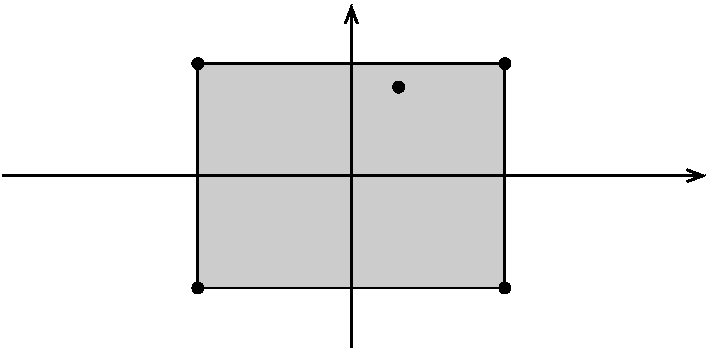
\includegraphics[height=50\unitlength]{hullm}}
\cell{71}{34}{c}{$\vc{x} = (x_1, x_2)$}
\cell{93}{41}{c}{$\vc{y} = (y_1, y_2)$}
\cell{90.5}{9}{c}{$(y_1, -y_2)$}
\cell{27.5}{9}{c}{$(-y_1, -y_2)$}
\cell{28.5}{41}{c}{$(-y_1, y_2)$}
% \cell{109}{22}{c}{$x$}
% \cell{57}{48}{c}{$y$}
\end{picture}
\caption{The vector $\vc{x}$ in the convex hull of the set $S$, as in the
  proof of Lemma~\ref{lemma:p-norm-elem}\bref{part:p-norm-mono}, shown for
  $n = 2$.}
\lbl{fig:hull}
\end{figure}
% 
But $\vc{x} \in \prod
[-y_i, y_i]$, and $\|\vc{s}\| = \|\vc{y}\|$ for each $\vc{s} \in S$ by
part~\bref{part:p-norm-pm}.  Hence, writing $\vc{x} = \sum
\lambda_{\vc{s}} \vc{s}$ and using the triangle inequality, 
\[
\|\vc{x}\|
\leq
\sum_{\vc{s} \in S} \lambda_{\vc{s}} \|\vc{s}\|
=
\sum_{\vc{s} \in S} \lambda_{\vc{s}} \|\vc{y}\|
=
\|\vc{y}\|.
\]

For~\bref{part:p-norm-one}, let $0 \leq m \leq n$.  We have
\[
\|\One_m\|
=
\|(\overbrace{\underbrace{1, \ldots, 1}_m,
0, \ldots, 0}^n) \|
\leq
\|\One_n\|,
\]
where the equality follows from the definition of system of norms and the
inequality follows from part~\bref{part:p-norm-mono}.
\end{proof}

\paragraph*{Step 2: finding $p$}
The idea now is that since $\|\One_n\|_p = n^{1/p}$ for all $p \in [1,
  \infty]$ and $n \geq 1$, we should be able to recover $p$ from
$\|\cdot\|$ by examining the sequence $\bigl(\|\One_n\|\bigr)_{n \geq 1}$.

Indeed, for all $m, n \geq 1$, multiplicativity gives
\[
\|\One_{mn}\| 
= 
\|\One_m \otimes \One_n\| 
=
\|\One_m\| \, \|\One_n\|.
\]
Moreover, Lemma~\ref{lemma:p-norm-elem}\bref{part:p-norm-one} implies that
the sequence $\bigl( \|\One_n\| \bigr)_{n \geq 1}$ is increasing.  Hence by
Theorem~\ref{thm:erdos-inc} applied to the sequence $\bigl( \log \|\One_n\|
\bigr)_{n \geq 1}$, there exists $c \geq 0$ such that $\|\One_n\| = n^c$
for all $n \geq 1$.  Now
\[
2^c
=
\|(1, 1)\|      
\leq
\|(1, 0)\| + \|(0, 1)\| 
=
2 \cdot \|(1)\| 
=
2 \cdot 1^c
=
2,
\]
so $c \in [0, 1]$.  Put $p = 1/c \in [1, \infty]$.  Then
\[
\|\One_n\| = n^{1/p} = \|\One_n\|_p
\]
for all $n \geq 1$.

We will show that $\|\vc{x}\| = \|\vc{x}\|_p$ for all $n \geq 0$ and
$\vc{x} \in \R^n$.  By definition of system of norms and
Lemma~\ref{lemma:p-norm-elem}\bref{part:p-norm-pm}, it is enough to prove
this when $\vc{x} \in (0, \infty)^n$.  The case $n = 0$ is trivial, so we
can also restrict to $n \geq 1$.

\paragraph*{Step 3: the case $p = \infty$}
This case needs separate handling, and is straightforward anyway.  We show
directly that if $p = \infty$ (that is, if $\|\One_n\| = 1$ for all $n \geq
1$) then $\|\cdot\| = \|\cdot\|_\infty$.

Let $\vc{x} \in (0, \infty)^n$, and choose $j$ such that $x_j =
\|\vc{x}\|_\infty$.  Then by
Lemma~\ref{lemma:p-norm-elem}\bref{part:p-norm-mono}, 
\[
\|\vc{x}\|
\leq
\|(x_j, \ldots, x_j)\|
=
x_j \|\One_n\|
=
x_j.
\]
But also 
\[
\|\vc{x}\|
\geq
\|(\underbrace{0, \ldots, 0}_{j - 1}, x_j, 
\underbrace{0, \ldots, 0}_{n - j})\|
=
\|(x_j)\|
=
x_j \|\One_1\|
=
x_j.
\]
Hence $\|\vc{x}\| = x_j = \|\vc{x}\|_\infty$, as required.

So, we may assume henceforth that $p \in [1, \infty)$.

\paragraph*{Step 4: exploiting the variational formula for $p$-norms}
We now use the formula for $p$-norms in Proposition~\ref{propn:p-norm-var}:
for $\vc{x} \in (0, \infty)^n$,
\[
\|\vc{x}\|_p 
=
\sup_{u > 0, \ r \geq 1} 
\Bigl(
u^r \, N(\vc{x}^{\otimes r}, u^r)^{1/p}
\Bigr)^{1/r}.
\]
(This is where the probability theory is used, as
Proposition~\ref{propn:p-norm-var} was derived from the variational
formula for moment generating functions.)  Since $m^{1/p} =
\|\One_m\|$ for all $m$, an equivalent statement is that
% 
\begin{equation}
\lbl{eq:p-norm-norm}
\|\vc{x}\|_p
=
\sup_{u > 0, \ r \geq 1}
\bigl\|
\bigl( 
N(\vc{x}^{\otimes r}, u^r) \mc u^r
\bigr)
\bigr\|^{1/r}.
\end{equation}
% 
Here we have used the notation $\mc$ introduced after
Definition~\ref{defn:decomp}.

The expression~\eqref{eq:p-norm-norm} for $\|\vc{x}\|_p$ has the feature
that it makes no mention of $p$.  We will use it to prove first that
$\|\vc{x}\| \geq \|\vc{x}\|_p$, then that $\|\vc{x}\| \leq \|\vc{x}\|_p$.

\paragraph{Step 5: the lower bound} 
Let $\vc{x} \in (0, \infty)^n$.  We show that $\|\vc{x}\| \geq
\|\vc{x}\|_p$.  By~\eqref{eq:p-norm-norm} and multiplicativity, it is
equivalent to show that
\[
\|\vc{x}^{\otimes r}\|
\geq
\bigl\|
\bigl( 
N(\vc{x}^{\otimes r}, u^r) \mc u^r
\bigr)
\bigr\|
\]
for all real $u > 0$ and integers $r \geq 1$.  But this is clear, since by
Lemma~\ref{lemma:p-norm-elem}\bref{part:p-norm-mono} and the definition of
system of norms, 
\[
\|\vc{x}^{\otimes r}\|
\geq 
\bigl\|\bigl(
\overbrace{
\underbrace{u^r, \ldots, u^r}_{N(\vc{x}^{\otimes r}, u^r)},
0, \ldots, 0}^{n^r}
\bigr)\bigr\|
=
\bigl\| \bigl(
N(\vc{x}^{\otimes r}, u^r) \mc u^r
\bigr) \bigr\|.
\]

\paragraph*{Step 6: the upper bound}
Let $\vc{x} \in (0, \infty)^n$.  We show that $\|\vc{x}\| \leq
\|\vc{x}\|_p$.  The argument is structurally very similar to the 
second part of the proof of Theorem~\ref{thm:cp}, and uses the tensor%
%
\index{tensor power trick} 
% 
power trick (Tao~\cite{TaoSR}, Section~1.9).

Let $\theta \in (1, \infty)$.  We will prove that $\|\vc{x}\| \leq
\theta\|\vc{x}\|_p$.  Since $\min_i x_i > 0$, we can choose an integer $d
\geq 1$ and real numbers $u_0, \ldots, u_d$ such that
\[
\min_i x_i = u_0 < u_1 < \cdots < u_d = \max_i x_i
\]
and $u_k/u_{k - 1} < \theta$ for all $k \in \{1, \ldots, d\}$.  

Let $r \geq 1$.  We have the vector $\vc{x}^{\otimes r} \in \R^{n^r}$, and
we define a new vector $\vc{y}_r \in \R^{n^r}$ by rounding up each
coordinate of $\vc{x}^{\otimes r}$ to the next element of the set $\{u_1^r,
\ldots, u_d^r\}$.  (Formally, define a map $f_r \from [u_0^r, u_d^r] \to
      [u_0^r, u_d^r]$ by $f_r(w) = u_k^r$, where $k \in \{1, \ldots, d\}$
      is least such that $w \leq u_k^r$. Then $\vc{y}_r$ is obtained from
      $\vc{x}^{\otimes r}$ by applying $f_r$ in each coordinate.)

By construction, $\vc{x}^{\otimes r} \leq \vc{y}_r$, and the number $n_{k,
  r}$ of coordinates of $\vc{y}_r$ equal to $u_k^r$ is at most
$N(\vc{x}^{\otimes r}, u_{k - 1}^r)$.  Hence
% 
\begin{align}
\|\vc{x}^{\otimes r}\|   &
\leq
\|\vc{y}_r\|    
\lbl{eq:ub-1} \\
&
=
\bigl\|
\bigl(
n_{1, r} \mc u_1^r, \ldots, n_{d, r} \mc u_d^r
\bigr)
\bigr\|
\lbl{eq:ub-2} \\
&
\leq
\sum_{k = 1}^d 
\bigl\|
\bigl(
(n_{1, r} + \cdots + n_{k - 1, r}) \mc 0,
n_{k, r} \mc u_k^r,
(n_{k + 1, r} + \cdots + n_{d, r}) \mc 0
\bigr)
\bigr\|
\lbl{eq:ub-3} \\
&
=
\sum_{k = 1}^d \| (n_{k, r} \mc u_k^r) \|
\lbl{eq:ub-4} \\
&
\leq
d \max_{1 \leq k \leq d} \| (n_{k, r} \mc u_k^r) \|
\lbl{eq:ub-5} \\
&
\leq
d \theta^r \max_{1 \leq k \leq d} \| (n_{k, r} \mc u_{k - 1}^r) \|
\lbl{eq:ub-6} \\
&
\leq
d \theta^r \max_{1 \leq k \leq d} 
\bigl\| \bigl(
N(\vc{x}^{\otimes r}, u_{k - 1}^r) \mc u_{k - 1}^r
\bigr) \bigr\|  
\lbl{eq:ub-7} \\
&
\leq
d \theta^r \|\vc{x}\|_p^r,
\lbl{eq:ub-8}
\end{align}
% 
where \eqref{eq:ub-1} is by
Lemma~\ref{lemma:p-norm-elem}\bref{part:p-norm-mono}, \eqref{eq:ub-2} is by
symmetry and definition of $n_{k, r}$, \eqref{eq:ub-3} is by the triangle
inequality, \eqref{eq:ub-4} is by definition of system of norms,
\eqref{eq:ub-5} is elementary, \eqref{eq:ub-6} is by hypothesis on $u_0,
\ldots, u_d$ and Lemma~\ref{lemma:p-norm-elem}\bref{part:p-norm-mono},
\eqref{eq:ub-7} uses Lemma~\ref{lemma:p-norm-elem}\bref{part:p-norm-one},
and~\eqref{eq:ub-8} follows from~\eqref{eq:p-norm-norm}.  Hence by
multiplicativity, 
\[
\|\vc{x}\| 
= 
\|\vc{x}^{\otimes r}\|^{1/r} 
\leq 
d^{1/r} \theta \|\vc{x}\|_p.
\]
This holds for all integers $r \geq 1$ and real numbers $\theta > 1$.
Letting $r \to \infty$ and $\theta \to 1$ gives $\|\vc{x}\| \leq
\|\vc{x}\|_p$, completing the proof of Theorem~\ref{thm:an}.

\begin{remark}
\lbl{rmk:an-diff} 
% 
The proof of Theorem~\ref{thm:an} originally given by Aubrun%
%
\index{Aubrun, Guillaume}
%
and Nechita%
%
\index{Nechita, Ion}
%
relied on both Cram\'er's theorem and the Legendre--Fenchel theorem.
Effectively, they used Cram\'er's theorem and convex duality to derive the
moment generating function formula of Theorem~\ref{thm:cp} in the specific
case required.

However, Cerf%
%
\index{Cerf, Rapha\"el}
% 
and Petit~\cite{CePe}%
%
\index{Petit, Pierre} 
% 
showed how the moment generating function formula can be proved without
these tools. (In fact, they used it as part of their proof of Cram\'er's
theorem.)  The proof of the moment generating function formula given in
Section~\ref{sec:mgfs} is similarly elementary.  Our proof of
Theorem~\ref{thm:an} works directly from the moment generating function
formula, and does not, therefore, need Cram\'er's theorem, the
Legendre--Fenchel theorem, or even the notion of convex conjugate.

Aubrun and Nechita went on to prove similar characterizations of the $L^p$
norms (Theorem~1.2 of~\cite{AuNe}) and the Schatten $p$-norms (their
Theorem~4.2).  The main focus of the article of Fern\'andez-Gonz\'alez,
Palazuelos and P\'erez-Garc\'{i}a~\cite{FGPPG} was also the $L^p$ norms
(their Theorem~3.1).  We do not discuss these results further.
\end{remark}
\index{Aubrun, Guillaume|)}
\index{Nechita, Ion|)}


\section{Multiplicative characterization of the power means}
\lbl{sec:mult-means}


From the multiplicative characterization of the $p$-norms, we derive a
multiplicative characterization of the power means of order at least~$1$.
It differs from the characterizations of power means in
Section~\ref{sec:w-mns} in that it does not assume modularity.  Instead, it
uses the multiplicativity condition of Definition~\ref{defn:w-mult}, as
well as a convexity axiom that provides the connection with norms.

\begin{defn}
\lbl{defn:mean-cvx}
A sequence of functions $\bigl( M \from \Delta_n \times [0, \infty)^n \to
[0, \infty) \bigr)_{n \geq 1}$ is \demph{convex}%
%
\index{convex!mean}%
\index{mean!convex} 
% 
if
\[
M\bigl( \vc{p}, \hlf(\vc{x} + \vc{y}) \bigr)
\leq
\max\bigl\{ M(\vc{p}, \vc{x}), M(\vc{p}, \vc{y}) \bigr\}
\]
for all $n \geq 1$, $\vc{p} \in \Delta_n$, and $\vc{x}, \vc{y} \in [0,
\infty)^n$. 
\end{defn}

\begin{example}
\lbl{eg:mean-mc}
% 
The power mean $M_t$ is multiplicative for all $t \in [-\infty, \infty]$
(Corollary~\ref{cor:pwr-mns-mult}).  If $t \in [1, \infty]$ then $M_t$ is
also convex.  To show this, it suffices to prove the inequality in
Definition~\ref{defn:mean-cvx} in the case where $\vc{p}$ has full support.
In that case, $M_t$ can be expressed in terms of $\|\cdot\|_t$ by the
formula
\[
M_t(\vc{p}, \vc{x})
=
\| \vc{p}^{1/t} \vc{x} \|_t
\]
($\vc{x} \in [0, \infty)^n$), where both the power and the product of
  vectors are defined coordinatewise.  Now, for $\vc{x}, \vc{y} \in [0,
    \infty)^n$,
% 
\begin{align*}
M_t\bigl( \vc{p}, \hlf(\vc{x} + \vc{y}) \bigr)  &
=
\bigl\| \hlf \vc{p}^{1/t}\vc{x} + \hlf \vc{p}^{1/t}\vc{y} \bigr\|_t     \\
&
\leq
\hlf \bigl\| \vc{p}^{1/t} \vc{x} \bigr\|_t 
+
\hlf \bigl\| \vc{p}^{1/t} \vc{y} \bigr\|_t      \\
&
=
\hlf \bigl( M_t(\vc{p}, \vc{x}) + M_t(\vc{p}, \vc{y}) \bigr)    \\
&
\leq
\max \bigl\{ M_t(\vc{p}, \vc{x}), M_t(\vc{p}, \vc{y}) \bigr\},
\end{align*}
% 
by the triangle inequality for $\|\cdot\|_t$.  Thus, $M_t$ is convex for $t
\in [1, \infty]$.   

On the other hand, $M_t$ is not convex for $t \in [-\infty, 1)$, since then
\[
M_t \Bigl( 
\bigl( \hlf, \hlf \bigr),
\hlf \bigl( (1, 0) + (0, 1) \bigr) 
\Bigr)
=
\hlf
\]
but
% 
\begin{align*}
\max \Bigl\{
M_t \bigl( \bigl(\hlf, \hlf\bigr), (1, 0) \bigr),
M_t \bigl( \bigl(\hlf, \hlf\bigr), (0, 1) \bigr)
\Bigr\} &
=
M_t\bigl( \bigl(\hlf, \hlf\bigr), (1, 0) \bigr)   \\
&
=
\begin{cases}
\bigl( \hlf \bigr)^{1/t}        &\text{if } t \in (0, 1),       \\
0                               &\text{if } t \in [-\infty, 0],
\end{cases}
\end{align*}
% 
which is strictly less than $1/2$.
\end{example}

The multiplicative characterization of the power means is as follows.  For
a review of the terminology used in~\bref{part:mcpm-condns}, see
Appendix~\ref{app:condns}.

\begin{thm}
\lbl{thm:mcpm}%
\index{power mean!characterization of!multiplicative}%
\index{power mean!characterization of!weighted on $[0, \infty)$}%
\index{multiplicative!characterization of power means}
%
Let $\bigl( M \from \Delta_n \times [0, \infty)^n \to [0, \infty) \bigr)_{n
\geq 1}$ be a sequence of functions.  The following are equivalent:
% 
\begin{enumerate}
\item 
\lbl{part:mcpm-condns}
$M$ is natural, consistent, increasing, multiplicative, and convex;

\item
\lbl{part:mcpm-form}
$M = M_t$ for some $t \in [1, \infty]$.
\end{enumerate}
\end{thm}

The proof follows shortly.

\begin{remarks}
\lbl{rmks:mcpm-matisos}
\begin{enumerate}
\item 
\lbl{rmk:mcpm-m-condns} 
We have already made some elementary inferences from combinations of the
properties in part~\bref{part:mcpm-condns} of the theorem.  In the proof of
Lemma~\ref{lemma:pwr-mns-elem} (p.~\pageref{p:lpme-pf}), we showed that
naturality implies symmetry, absence-invariance and repetition.  Since $M$
is increasing, Lemma~\ref{lemma:transfer} then implies that $M$ also has
the transfer property.  Moreover, $M$ is homogeneous, since for all $\p \in
\Delta_n$, $\vc{x} \in [0, \infty)^n$, and $c \in [0, \infty)$,
% 
\begin{align*}
M(\vc{p}, c\vc{x})      &
=
M\bigl(\vc{u}_1 \otimes \vc{p}, (c) \otimes \vc{x}\bigr)        \\
&
=
M\bigl( \vc{u}_1, (c) \bigr) M(\vc{p}, \vc{x})  \\
&
=
c M(\vc{p}, \vc{x}), 
\end{align*}
% 
by definition of $\otimes$, multiplicativity, and consistency.

\item
\lbl{rmk:mcpm-m-cons}
Theorem~\ref{thm:mcpm} first appeared as Theorem~1.3 of
Leinster~\cite{MCPM}.  There, the result was stated with a superficially
weaker consistency axiom: that $M(\vc{u}_1, (x)) = x$ for all $x \in [0,
\infty)$.  But in the presence of the naturality property, this easily
implies full consistency: for naturality implies repetition (as just
noted), which in turn implies that
\[
M\bigl(\vc{p}, (x, \ldots, x)\bigr)
=
M\bigl((p_1 + \cdots + p_n), (x)\bigr)
=
M\bigl(\vc{u}_1, (x)\bigr)
=
x
\]
for all $\p \in \Delta_n$ and $x \in [0, \infty)$. 
\end{enumerate}
\end{remarks}

We now embark on the proof of Theorem~\ref{thm:mcpm}.
Certainly~\bref{part:mcpm-form} implies~\bref{part:mcpm-condns}, by
Lemmas~\ref{lemma:pwr-mns-nat}, \ref{lemma:pwr-mns-con}
and~\ref{lemma:pwr-mns-inc}, Corollary~\ref{cor:pwr-mns-mult}, and
Example~\ref{eg:mean-mc}.  For the converse, and \femph{for the rest of
  this section}, let $M$ be a sequence of functions satisfying the
conditions in Theorem~\ref{thm:mcpm}\bref{part:mcpm-condns}.  We will prove
that $M = M_t$ for some $t \in [1, \infty]$.

\paragraph*{Step 1: finding $t$} 
The observation behind this step is that 
\[
M_t \bigl((p, 1 - p), (1, 0)\bigr) = p^{1/t}
\]
for all $p \in (0, 1)$. 

Define a function $f \from (0, 1) \to [0, \infty)$ by
\[
f(p) = M\bigl( (p, 1 - p), (1, 0) \bigr).
\]
By multiplicativity and repetition (proved in
Remark~\ref{rmks:mcpm-matisos}\bref{rmk:mcpm-m-condns}),
% 
\begin{align*}
f(p)f(r)        &
=
M\bigl( (p, 1 - p), (1, 0) \bigr)
\cdot
M\bigl( (r, 1 - r), (1, 0) \bigr)       \\
&
=
M\bigl( 
(p, 1 - p) \otimes (r, 1 - r), \, (1, 0) \otimes (1, 0)
\bigr)  \\
&
=
M\Bigl(
\bigl(pr, p(1 - r), (1 - p)r, (1 - p)(1 - r)\bigr), \, 
(1, 0, 0, 0)
\Bigr)  \\
&
=
M\bigl( (pr, 1 - pr), \, (1, 0) \bigr)  \\
&
=
f(pr)
\end{align*}
% 
for all $p, r \in (0, 1)$.  By transfer
(Remark~\ref{rmks:mcpm-matisos}\bref{rmk:mcpm-m-condns}),  $f$ is
increasing.  If $f(r) = 0$ for some $r \in (0, 1)$ then for all $p \in (0,
1)$, 
\[
f(p)
=
f(p/r) f(r)
=
0 
=
p^\infty.
\]
If not, then $f$ defines an increasing multiplicative function $(0, 1) \to
(0, \infty)$, so by Corollary~\ref{cor:cauchy-mult-01}, there is some
constant $c \in [0, \infty)$ such that $f(p) = p^c$ for all $p \in (0, 1)$.
  So in either case, there is a constant $c \in [0, \infty]$ such that
  $f(p) = p^c$ for all $p \in (0, 1)$.  But
\[
f\bigl(\hlf\bigr)
=
M\bigl( \vc{u}_2, (1, 0) \bigr)
=
M\bigl( \vc{u}_2, (0, 1) \bigr)
\]
by symmetry, so 
% 
\begin{align*}
\bigl(\hlf\bigr)^c        &
=
f\bigl(\hlf\bigr) \\
&
=
\max\Bigl\{
M\bigl( \vc{u}_2, (1, 0) \bigr),
M\bigl( \vc{u}_2, (0, 1) \bigr) 
\Bigr\} \\
&
\geq
M\bigl( \vc{u}_2, \bigl(\hlf, \hlf\bigr) \bigr)
=
\hlf
\end{align*}
% 
by convexity and consistency.  It follows that $c \in [0, 1]$.  Put $t =
1/c \in [1, \infty]$: then
%  
\begin{equation}
\lbl{eq:agree-10}
M\bigl( (p, 1 - p), (1, 0) \bigr)
=
p^{1/t}
=
M_t \bigl( (p, 1 - p), (1, 0) \bigr)
\end{equation}
% 
for all $p \in (0, 1)$.

\paragraph*{Step 2: constructing a system of norms} 
Here we take our inspiration from the relationship
\[
\|\vc{x}\|_t
=
n^{1/t} 
M_t\bigl(
\vc{u}_n, (\mg{x_1}, \ldots, \mg{x_n})
\bigr)
\]
($\vc{x} \in \R^n$) between the $t$-norm and the power mean of order $t$.

For each $n \geq 1$, define a function $\|\cdot\| \from \R^n \to [0,
  \infty)$ by
\[
\|\vc{x}\|
=
n^{1/t} 
M\bigl(
\vc{u}_n, (\mg{x_1}, \ldots, \mg{x_n})
\bigr)
\]
($\vc{x} \in \R^n$).  To cover the case $n = 0$, let $\|\cdot\| \from \R^0
\to [0, \infty)$ be the function whose single value is $0$.  The next few
lemmas show that $\|\cdot\|$ is a multiplicative system of norms.

\begin{lemma}
\lbl{lemma:mcpm-pwr}
$n^{-1/t} = M\bigl(\vc{u}_n, (1, 0, \ldots, 0)\bigr)$ for all $n \geq 1$.  
\end{lemma}

\begin{proof}
By the defining property of $t$ (equation~\eqref{eq:agree-10}) and the
repetition property of $M$, both sides are equal to $M\bigl( (1/n, 1 -
1/n), (1, 0) \bigr)$.
\end{proof}

\begin{lemma}
\lbl{lemma:mcpm-yes-norm}
For each $n \geq 0$, the function $\|\cdot\| \from \R^n \to [0, \infty)$
  is a norm.
\end{lemma}

\begin{proof}
This is trivial when $n = 0$; suppose that $n \geq 1$.  We verify the three
conditions in the definition of norm (Definition~\ref{defn:norm}).

First, we have to prove that if $\vc{0} \neq \vc{x} \in \R^n$ then
$\|\vc{x}\| \neq 0$.  We may assume by symmetry that $x_1 \neq 0$, and then
% 
\begin{align*}
\|\vc{x}\|      &
\geq
n^{1/t} M\bigl(\vc{u}_n, (\mg{x_1}, 0, \ldots, 0) \bigr)   \\
&
=
n^{1/t} \mg{x_1} M\bigl(\vc{u}_n, (1, 0, \ldots, 0)\bigr)  \\
&
=
\mg{x_1} > 0
\end{align*}
% 
by definition of $\|\vc{x}\|$, the increasing and homogeneity properties of
$M$, and 
% since $M$ is increasing and homogeneous, and using
Lemma~\ref{lemma:mcpm-pwr}. 

The homogeneity of $M$ implies that $\|c\vc{x}\| = \mg{c}\,\|\vc{x}\|$ for
all $\vc{x} \in \R^n$ and $c \in \R$.

It remains to prove the triangle inequality, which we do in stages.  First
let $\vc{x}, \vc{y} \in \R^n$ with $\|\vc{x}\|, \|\vc{y}\| \leq 1$ and
$x_i, y_i \geq 0$ for all $i$.  Using the convexity of $M$,
% 
\begin{align*}
\bigl\| \hlf \vc{x} + \hlf \vc{y} \bigr\|       &
=
n^{1/t} M\bigl( \vc{u}_n, \hlf(\vc{x} + \vc{y}) \bigr)  \\
&
\leq
n^{1/t} \max\bigl\{ M(\vc{u}_n, \vc{x}), M(\vc{u}_n, \vc{y}) \bigr\}    \\
&
=
\max \bigl\{ \|\vc{x}\|, \|\vc{y}\| \bigr\}    \\
&
\leq
1.
\end{align*}
% 
It follows that
% 
\begin{equation}
\lbl{eq:tri-cvx}
\|\lambda \vc{x} + (1 - \lambda) \vc{y}\| \leq 1
\end{equation}
% 
for all dyadic rationals $\lambda = k/2^\ell \in [0, 1]$, by induction on
$\ell$.  We now show that~\eqref{eq:tri-cvx} holds for all $\lambda \in [0,
  1]$.  Indeed, given $\lambda \in [0, 1]$ and $\epsln > 0$, we can choose
a dyadic rational $\lambda' \in [0, 1]$ such that
\[
\lambda \leq (1 + \epsln) \lambda',
\qquad
1 - \lambda \leq (1 + \epsln)(1 - \lambda'),
\]
and then
% 
\begin{align*}
\| \lambda \vc{x} + (1 - \lambda) \vc{y} \|   &
\leq
\| 
(1 + \epsln) \lambda' \vc{x} + (1 + \epsln)(1 - \lambda') \vc{y} 
\| \\
&
=
(1 + \epsln) \| \lambda' \vc{x} + (1 - \lambda') \vc{y} \|    \\
&
\leq
1 + \epsln,
\end{align*}
% 
where in the first inequality, we used the assumptions that $M$ is
increasing and $x_i, y_i \geq 0$.  This holds for all $\epsln > 0$, proving
the claimed inequality~\eqref{eq:tri-cvx}.

Now take any $\vc{x}, \vc{y} \in \R^n$ with $x_i, y_i \geq 0$ for all $i$.
We will prove that 
% 
\begin{equation}
\lbl{eq:tri-mn}
\|\vc{x} + \vc{y}\| \leq \|\vc{x}\| + \|\vc{y}\|.
\end{equation}
% 
This is immediate if $\vc{x} = \vc{0}$ or $\vc{y} = \vc{0}$.  Supposing
otherwise, put
\[
\hat{\vc{x}} = \frac{\vc{x}}{\|\vc{x}\|},
\qquad
\hat{\vc{y}} = \frac{\vc{y}}{\|\vc{y}\|},
\qquad
\lambda = \frac{\|\vc{x}\|}{\|\vc{x}\| + \|\vc{y}\|}.
\]
Then $\|\hat{\vc{x}}\| = \|\hat{\vc{y}}\| = 1$, so by 
inequality~\eqref{eq:tri-cvx} applied to $\hat{\vc{x}}$, $\hat{\vc{y}}$ and
$\lambda$, 
\[
\|\vc{x} + \vc{y}\|     
=
( \|\vc{x}\| + \|\vc{y}\| ) \,
\| \lambda \hat{\vc{x}} + (1 - \lambda) \hat{\vc{y}} \|     
\leq
\|\vc{x}\| + \|\vc{y}\|.
\]

Finally, take any $\vc{x}, \vc{y} \in \R^n$.  To prove the triangle
inequality~\eqref{eq:tri-mn}, put $\vc{x}' = (\mg{x_1}, \ldots, \mg{x_n})$
and $\vc{y}' = (\mg{y_1}, \ldots, \mg{y_n})$.  Then $\|\vc{x}\| =
\|\vc{x}'\|$ and $\|\vc{y}\| = \|\vc{y}'\|$ by definition of $\|\cdot\|$,
and
\[
\|\vc{x} + \vc{y}\| \leq \|\vc{x}' + \vc{y}'\|
\]
since $M$ is increasing.  By the inequality proved in the previous
paragraph, 
\[
\|\vc{x}' + \vc{y}'\| \leq \|\vc{x}'\| + \|\vc{y}'\|,
\]
and the triangle inequality~\eqref{eq:tri-mn} follows.
\end{proof}

\begin{lemma}
\lbl{lemma:mcpm-yes-sys}
$\|\cdot\|$ is a multiplicative system of norms.  
\end{lemma}

\begin{proof}
We have just shown that $\|\cdot\|$ is a norm on $\R^n$ for each individual
$n$.  Symmetry of $M$ implies symmetry of $\|\cdot\|$, so to show that
$\|\cdot\|$ is a system of norms, it suffices to prove that
% 
\begin{equation}
\lbl{eq:sys-pad}
\| (x_1, \ldots, x_n) \|
=
\| (x_1, \ldots, x_n, 0) \|
\end{equation}
% 
for all $n \geq 1$ and $\vc{x} \in \R^n$.  By definition of $\|\cdot\|$ and
Lemma~\ref{lemma:mcpm-pwr}, equation~\eqref{eq:sys-pad} is equivalent to
\[
\frac{M\bigl( \vc{u}_n, (\mg{x_1}, \ldots, \mg{x_n}) \bigr)}%
{M\bigl(\vc{u}_n, (1, 0, \ldots, 0) \bigr)}
=
\frac{M\bigl( \vc{u}_{n + 1}, (\mg{x_1}, \ldots, \mg{x_n}, 0) \bigr)}%
{M\bigl(\vc{u}_{n + 1}, (1, 0, \ldots, 0, 0) \bigr)},
\]
or equivalently,
% 
\begin{align*}
&
M\bigl( \vc{u}_{n + 1}, (1, 0, \ldots, 0, 0) \bigr)
\cdot
M\bigl( \vc{u}_n, (\mg{x_1}, \ldots, \mg{x_n}) \bigr) \\
=\ 
&
M\bigl( \vc{u}_n, (1, 0, \ldots, 0) \bigr)
\cdot
M\bigl( \vc{u}_{n + 1}, (\mg{x_1}, \ldots, \mg{x_n}, 0) \bigr).
\end{align*}
% 
But by multiplicativity and symmetry, both sides are equal to
\[
M\bigl(
\vc{u}_{n(n + 1)},
(\mg{x_1}, \ldots, \mg{x_n}, \underbrace{0, \ldots, 0}_{n^2})
\bigr),
\]
proving~\eqref{eq:sys-pad}.

Finally, the system of norms $\|\cdot\|$ is multiplicative, by
multiplicativity of $M$.
\end{proof}

\paragraph*{Step 3: using the norm theorem}
It now follows from Theorem~\ref{thm:an} that $\|\cdot\| = \|\cdot\|_s$ for
some $s \in [1, \infty]$.  Thus, $\|\vc{x}\|_s = n^{1/t} M(\vc{u}_n,
\vc{x})$ for all $n \geq 1$ and $\vc{x} \in [0, \infty)^n$.  But also,
  $\|\vc{x}\|_s = n^{1/s} M_s(\vc{u}_n, \vc{x})$, so
\[
n^{1/t} M(\vc{u}_n, \vc{x})
=
n^{1/s} M_s(\vc{u}_n, \vc{x})
\]
for all $n \geq 1$ and $\vc{x} \in [0, \infty)$.  Putting $n = 2$ and
  $\vc{x} = (1, 1)$, and using the consistency of both $M$ and $M_s$, gives
  $s = t$.  Hence for all $n \geq 1$ and $\vc{x} \in [0, \infty)^n$,
\[
M(\vc{u}_n, \vc{x})
% =
% n^{-1/t} \|\vc{x}\|_t
=
M_t(\vc{u}_n, \vc{x}).
\]

\paragraph*{Step 4: arbitrary weights}
We have now shown that $M(\vc{u}_n, -) = M_t(\vc{u}_n, -)$ for all $n \geq
1$.  To extend the equality to arbitrary weights, we use
Proposition~\ref{propn:u-to-w}, taking $M' = M_t$ there.  The hypotheses of
that proposition are satisfied, by
Remark~\ref{rmks:mcpm-matisos}\bref{rmk:mcpm-m-condns} and
Lemma~\ref{lemma:pwr-mns-cts-px}\bref{part:pwr-mns-cts-px-1}.  Hence $M =
M_t$.

This completes the proof of Theorem~\ref{thm:mcpm}, the multiplicative
characterization of the power means.







